



\chapter{Implementação}

Neste capitulo será apresentado ....

kkkkkkkkkDurante o desenvolvimento um software pressupõe-se que os seus intervenientes sigam determinadas metodologia para o seu programa possa revolucionar a vida de um grupo em especifico ou até mesmo da sociedade. 
Durante o desenvolvimento um software pressupõe-se que os seus intervenientes sigam determinadas metodologia para o seu programa possa revolucionar a vida de um grupo em especifico ou até mesmo da sociedade. kkkkkkkkk


















\section{Sistema de informação}


trigger..



\subsection{\ac{API}}

\subsection{Aplicação web}





\subsection{Aplicação mobile}




\subsection{\textit{Deploy} do projecto}


https://jee-appy.blogspot.com.tr/2015/04/deploy-django-project-on-apache-using.html

Caracteristicas da maquina virtual

Description:	Ubuntu 14.04.1 LTS
64 bitsRAM 2GB 






\newpage
\section{Simulação em hardware}

Nesta secção pretende-se explicar a implementação a nível de \textit{software} no contexto desta simulação para cada um dos micro-controladores. 


\subsection{Arduino}

No que diz respeito ao Arduino Nano (\ac{SM}), numa fase inicial,  procedeu-se à ligação dos diversos componentes anteriormente apresentados na \textit{breadboard} tal como se encontra apresentado no Anexo \ref{interlapd}. Para auxiliar o desenvolvimento de \textit{software} foi utilizada a versão 1.8.1 do \ac{IDE} do próprio Arduino\footnote{https://www.arduino.cc/en/Main/Software}.  

Seguidamente apresenta-se a implementação necessária a nível de sensores e de comunicação. 

\subsection{Sensores}



Foram desenvolvidos os seguintes métodos que permitem aceder aos valores lidos de cada um dos sensores. Para além disso, foi criado um método que permite alterar o estado do válvula para transferência de água. 

\begin{itemize}
	\item \texttt{int readTemperature(int port)}: é efetuada uma leitura no porto analógico. Após a leitura este é convertido para ºC (graus Celsius)
	
	\item \texttt{long readLuminosity(int port)}: 
	
	\item \texttt{int readWaterValve(int port)}: é efetuada uma leitura no porto digital através do método \texttt{digitalRead}. 
	
	\item \texttt{int readWaterLevel(int port)}: é efetuada uma leitura no porto digital através do método \texttt{digitalRead}.
	
	
	\item \texttt{void setWaterValve(int port, int state)}: se a variável \texttt{state} for 1 então o porto é colocado a \texttt{HIGH} (1) através do método \texttt{digitalWrite}, caso contrário é colocado a \texttt{LOW} (0)
	
\end{itemize}

Inicialmente procedeu-se à leitura de cada sensor de forma individual de modo a garantir o seu total funcionamento. Sempre que é feita um pedido de leitura dos sensores pelo \ac{CM} os valores são enviados com o seguinte formato: 

\begin{equation} 
\label{eq:someequation}
\texttt{<temperatura>;<nível\_água>;<luminosidade>;<estado\_válvula>}
\end{equation}

\subsection{Comunicação}


Numa primeira fase procedeu-se à comunicação entre o \ac{SM} e \ac{CM} através de porta série. Seguidamente resolveu-se incorporar o módulo bluetooth de modo a tornar cada módulo independente. De módulo de interagir com o módulo bluetooth utilizou-se o package \texttt{SoftwareSerial.h} disponível no Arduino. Decidiu-se que caso o módulo bluetooth recebesse valores de 0 a 2 tinha diferentes comportamentos: 

\begin{itemize}
	\item \textbf{0}: ativação (ligar) da válvula; 
	\item \textbf{1}: desativação (desligar) da válvula; 
	\item \textbf{2}: recebe dados obtidos pelos sensores no formato definido em (\ref{eq:someequation})
\end{itemize}

Antes de proceder à implementação de envio e receção de dados por bluetooth no Raspberry Pi 3 optou-se por testar este mecanismo através de uma aplicação Android existente na \textit{Play Store} chamada de \textit{Bluetooth Terminal HC-05}\footnote{https://play.google.com/store/apps/details?id=project.bluetoothterminal}

\subsubsection{Raspberry Pi}


\subsubsection{Comunicação}


Como é possível observar na figura \ref{esquemcomm}, para a comunicação no Raspberry Pi (\ac{CM}) entre o Arduino (\ac{SM}) foi utilizado o modulo interno de bluetooth 4.1 que este incorpora no seu hardware. Para tal, foi desenvolvido um \textit{script} em Python que permite o seguinte: 


\begin{enumerate}
	\item Verificar dispositivos bluetooth disponíveis
	\item Estabelecer conexão com módulo HC-06 através de um socket para comunicação utilizando para isso o \textit{package} \texttt{socket} do python. 
	\item Aceder à API para verificar estado da válvula de admissão de águas e enviá-lo através do socket utilizando o método \texttt{send()} 
	\item No caso se ser enviado o digito 1 a válvula será aberta, enquanto que se for enviado o digito 2 a válvula é fechada. 
	\item No caso de ser enviado o digito 2, o socket ficará à espera de receber os dados lidos pelos sensores, utilizando para isso o método \texttt{recv()}
	\item Após receber os dados lidos, é efetuado algum processamento para que os dados sejam enviados através da API. 
	\item Todos os pontos 3 a 6 são repetidos com um atraso igual ao seding time definido o sensor module na dashboard. 
	
\end{enumerate}

Para permitir o acesso aos recursos do sistema Bluetooth foi utilizada uma extensão (\textit{package}) do Python denominado de \textit{pybluez}\footnote{https://github.com/karulis/pybluez}. 




\subsection{Considerações finais}


>1 fase testar coneccao arduino to rasp via porta serie; foi criado um script em python para processar info e enviar para o servidor através da API 

>2 fase : necessidade de tornar um módulo isolado sem necessidade de fio; foi testado um modulo wifi e bluetooth; 

>neste contexto modulo wifi nao!... pretende-se que os sensor moduels sejam de baixo custo e low power. foi utilizado um modulo bluetooth; foi testada a conexao da comm bluetooth através de uma client disponveil na google play bluetooth terminal HC-05 


> 
pq nao foi usado um sensor de salinidade? nao havia orçamento.. 










\section{Sistema de deteção de intrusos}


No contexto desta dissertação houve necessidade de implementar um sistema de video-stream que permitisse detetar intrusos, maioritariamente pessoas ou animais de grande porte, que possam invadir as quintas onde se produz salicornia. Esta necessidade prende-se essencialmente com elevado custo do hardware do sistema de monitorização e também de eventuais instrumentos de elevado custo necessários ao cultivo desta espécie (e.g. geradores, maquinas elétricas para poda etc).

Neste capitulo é descrita a tecnologia de processamento de imagem utilizada tal como o algoritmo disponibilizado pela mesma. Apresenta-se a implementação deste mecanismo e os testes necessários. 


\subsection{Biblioteca de processamento de imagem: OpenCV}

O OpenCV, também conhecido por \textit{Open Source Computer Vision Library}, é uma biblioteca de software de visão por computador de código \textit{open source} (figura \ref{opencvlogo}). OpenCV foi construído para fornecer uma infra-estrutura comum para aplicações de visão computacional e para criar o uso da perceção da máquina nos produtos comerciais.

A biblioteca possui mais de 2500 algoritmos otimizados, que inclui um conjunto abrangente de algoritmos clássicos e avançados de visão computacional e algoritmos de \textit{machine learning}. Esses algoritmos podem ser usados para detectar e reconhecer rostos, identificar objetos, classificar ações humanas em vídeos, detetar movimentos numa câmara, seguir um objetos em movimento, produzir nuvens de pontos 3D de câmaras estéreo, entre outros.
OpenCV tem mais de 47 mil pessoas na comunidade de usuários e o número estimado de downloads superior a 7 milhões. A biblioteca é amplamente utilizada em empresas e grupos de pesquisa \cite{Itseez}.

O OpenCV é usado principalmente em aplicações de visão em tempo real. Esta biblioteca tem interfaces nas mais diversas linguagens: C++, C, Python, Java e MATLAB, embora seja nativamente escrito em C. OpenCV tem suporte para Windows, Linux e Mac OS\cite{Itseez}. 

\begin{figure}[!htb]
	\centering
	
\includegraphics[width=0.5\linewidth]{img/vision/opencv_logo.jpg}
	\caption{Logótipo OpenCV}
	\label{opencvlogo}
\end{figure}


\textbf{Conclusoes} 

Desde logo a escolha da tecnologia para processamento de imagem recaiu sobre o opencv não apenas por ser uma biblioteca bastante popular e possuir bastantes algoritmos implementados mas também por eu próprio possuir já algum background e projetos desenvolvidos neste neste contexto.


Pretendeu-se que este processamento fosse implementado em material já adquirido sem necessidade de gastos. Optou-se então por utilizar um \textit{Raspberry Pi} que juntamente com um \textit{Raspberry Pi camera module} (figura \ref{raspicam}) permitirá a aquisição de imagem e servirá também como \textit{controller module} ao sistema de aquisição de dados. 


\begin{figure}[!htb]
	\centering
	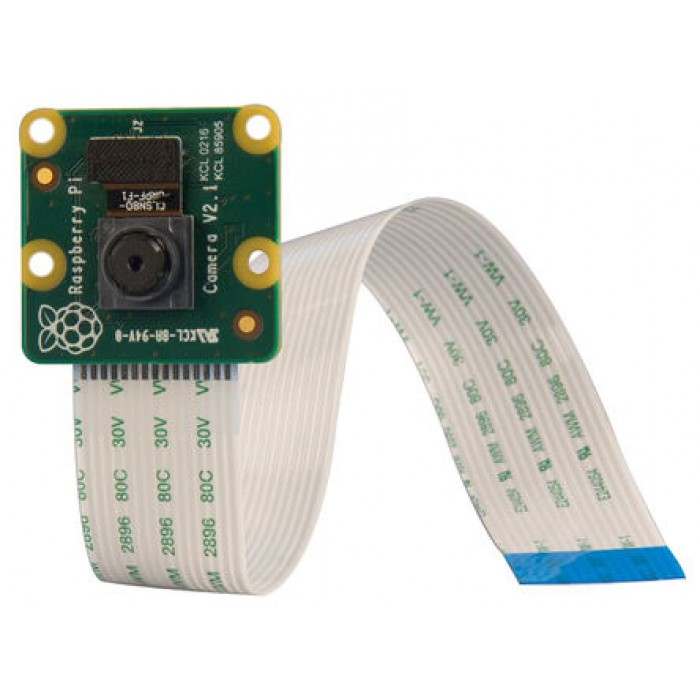
\includegraphics[width=0.3\linewidth]{img/hardware/camera_v2.jpg}
	\caption{Raspberry Pi Camera Board V2 8MP 1080p}
	\label{raspicam}
\end{figure}


Eis algumas das características principais do Raspberry Pi Camera Board V2:

\begin{itemize}
	\item lente de foco fixo on-board
	\item 150 milímetros CSI cabo da câmara incluída
	\item 8 megapixels do sensor com capacidade de resolução nativa de 3.280 imagens estáticas de pixels x 2464
	\item Suporta 1080p30, 720p60 e 640x480p90 vídeo
	\item Tamanho 25 milímetros x 23 milímetros x 9 mm
	\item Peso pouco mais de 3 g
	\item Liga-se à placa de framboesa Pi por meio de um cabo de fita curta (fornecido)
	\item Camera v2 é compatível com a última versão do Raspbian, sistema operacional preferido do Raspberry Pi
\end{itemize}


No que toca ao desenvolvimento, optou-se por utilizar o package picamera. Este pacote fornece  uma interface em Python (disponível para qualquer versão) para o módulo de câmara Raspberry Pi\footnote{http://picamera.readthedocs.io/en/release-1.13/}, permitindo uma fácil interação entre a aquisição da imagem e respetivo processamento. Neste contexto optou-se obviamente por utilizar a interface Python da biblioteca do OpenCV.



\subsection{Algoritmos de deteção de intrusos}
% artigo http://lear.inrialpes.fr/people/triggs/pubs/Dalal-cvpr05.pdf

De modo a estudar alguns algoritmos de deteção de pessoas foram estudados alguns artigos neste contexto. 


Para a resolução deste problema foi efetuados 


HOGDescriptor: classe que implementa um histograma de gradientes orientado ( [Dalal2005] ) detetor de objetos. 

hog = cv2.HOGDescriptor()
hog.setSVMDetector(cv2.HOGDescriptor\_getDefaultPeopleDetector())




Usado biblioteca do opencv que permite detectar 
HOGDescriptor


Deteção de intrusos: 

http://www.pyimagesearch.com/2015/11/09/pedestrian-detection-opencv/



versão simplificada: http://www.pyimagesearch.com/2015/02/16/faster-non-maximum-suppression-python/



Servidor em falsk 


deploy 
https://iotbytes.wordpress.com/python-flask-web-application-on-raspberry-pi-with-nginx-and-uwsgi/



Dataset: %http://www.robots.ox.ac.uk/ActiveVision/Research/Projects/2009bbenfold_headpose/project.html


é usado um detector HOG juntamente com um classificador linear SVM 





parametros do método detectMultiScale do opencv 

\begin{itemize}
	\item \texttt{img}: parâmetro obrigatório. 
	\item \texttt{hitThreshold}: parâmetro opcional. 
	\item \texttt{winStride}: parâmetro opcional. 
	\item \texttt{padding}: parâmetro opcional.  Os valores típicos para preenchimento incluem  (8, 8) ,  (16, 16) ,  (24, 24) , e  (32, 32) .
	
	
	\item \texttt{scale}: parâmetro opcional. 
	\item \texttt{finalThreshold}: parâmetro opcional. 
	\item \texttt{useMeanShiftGrouping}: parâmetro opcional. 
\end{itemize}





Neste contexto apenas foram utilizados os seguintes parâmetros winStride, scale, padding. 



\subsection{Testes}

Foram considerados 4 frames de imagens .... e no apêndice X




\subsection{Implementação}


%\subsection{Flask}

Flask é considerada uma microframework web desenvolvida em Python e baseado nas bibliotecas WSGI Werkzeug e Jinja2. Escolhi esta microframework pois pretende-se que esta seja executada num microcontrolador com baixos recursos. Para além disso, considera-se ser de fácil aprendizagem relativamente ao Django (já abordado na capitulo XX) e com uma ótima documentação. 




%\subsection{Servidor web NGNIX}

\section{Considerações finais}





